\chapter{Rendering Pipeline}
\begin{figure}[H]
	\centering
	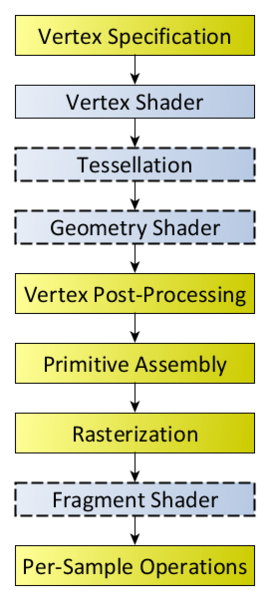
\includegraphics[scale=0.4]{imagens/openglPipeline.png}
	\caption{\small \textit{Rendering pipeline} OpenGL (Fonte: OPENGL, 2016b)}
	\label{fig:glpipeline}
\end{figure}

O processo de execução de um programa que exibe resultados em um monitor gráfico requer uma série de etapas, com grande quantidade de cálculos (CLEMENTS, 2014). Assim como na CPU (\textit{Central Processing Unit}, Unidade de Processamento Central), que realiza o processamento geral do computador, a GPU (\textit{Graphics Processing Unit}, Unidade de Processamento Gráfico), também se beneficia de \textit{pipeline}.

Tal processo é definido pela execução paralela de múltiplas etapas, diminuindo a ociosidade do \textit{hardware} e aumentando a taxa de saída de dados (\textit{throuput}) (SHEN e LIPASTI, 2013). Logo que uma primeira instrução é finalizada em uma etapa, uma segunda pode iniciar, desde que não possua outras dependências.

A primeira etapa programável de processamento é o \textit{vertex shader}, sendo também a única obrigatória. Sua função é efetuar cálculos, tendo apenas um vértice como entrada e saída de dados (OPENGL, 2016b). Para funcionar corretamente, o programador deve especificar a entrada, chamada de \textit{vertex attribute}. Isto é feito através da chamada de funções específicas do OpenGL, utilizando como parâmetros o nome dos atributos.

\begin{lstlisting}[language=glsl,
label={lst:vertexshader},
caption="Exemplo de \textit{vertex shader}"]
	#version 330
	layout (location = 0) in vec3 position;
	layout (location = 1) in vec3 normal;
	
	out vec3 Normal;
	out vec3 FragPos;
	
	uniform mat4 model;
	uniform mat4 view;
	uniform mat4 projection;
	
	void main()
	{
		gl_Position = projection * view *  model * vec4(position, 1.0f);
		FragPos = vec3(model * vec4(position, 1.0f));
		Normal = mat3(transpose(inverse(model))) * normal;  
	} 
}
\end{lstlisting}

No código \ref{lst:vertexshader}, podemos notar as entradas definidas por \lstinline{layout(location = #)} e as saídas por \lstinline{out}, que serão utilizadas na próxima etapa do \textit{pipeline}. Devido a natureza independente dos vértices, estes podem ser processados paralelamente em alta velocidade, fazendo uso dos múltiplos núcleos da GPU (AKENINE-MÖLLER et al, 2016).

\begin{figure}[H]
	\centering
	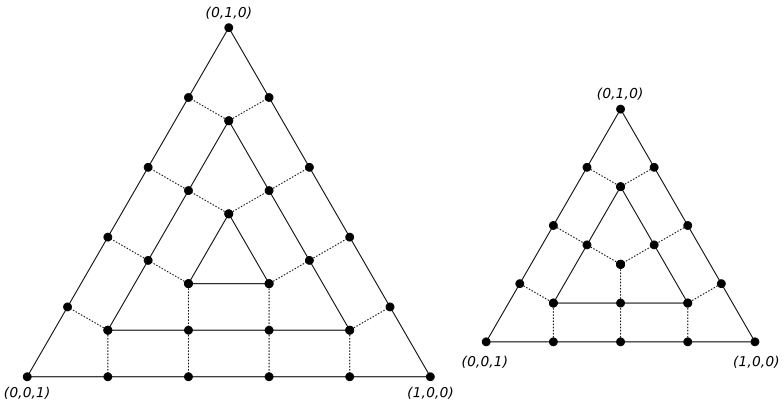
\includegraphics[scale=0.5]{imagens/tesselation.png}
	\caption{\small \textit{Tesselation} (Fonte: OPENGL, 2016c)}
	\label{fig:tesselation}
\end{figure}

A próxima etapa de processamento é chamada de \textit{tesselation}, que consiste de duas etapas programáveis opcionais e uma fixa. Este estágio atua sobre \textit{patches}, uma primitiva determinada por uma certa quantidade de vértices especificada pelo programador. Primitivas são tipos de dados processados no OpenGL, representados por sequências de vértices, como pontos, linhas, triângulos e sequências dos dois últimos (OPENGL, 2016c).

Na primeira operação, o \textit{tesselation control shader} recebe um \textit{patch} de entrada e emite outro de saída, podendo determinar as operações a serem efetuadas a cada vértice e a cada \textit{patch}. Através dele é possível aplicar subdivisões de geometria diretamente da GPU (BAILEY e CUNNINGHAM, 2012), por exemplo, para alterar a quantidade de vértices de um objeto. Com uma quantidade maior, o nível de detalhamento da superfície também aumenta. Pode ser usado para criar o efeito de um objeto sendo visto de diferentes distâncias, ao mesmo tempo que economiza o processamento de detalhes desnecessários. 

Caso o \textit{tesselation evaluation shader} esteja presente, os dados são transferidos para a etapa fixa \textit{tesselation primitive generation}. Sua função é transformar os \textit{patches} gerados anteriormente em primitivas, de acordo com os valores especificados pelo \textit{shader}. Por último, o \textit{evaluation shader} gera efetivamente os novos vértices e seus atributos.

No próximo estágio opcional, o \textit{geometry shader}, cada primitiva pode ser processada novamente, gerando nenhuma ou mais primitivas. Uma de suas características importantes é a capacidade de executar múltiplas vezes para a mesma primitiva, gerando resultados que podem ser utilizados em diferentes funções. Por exemplo, processar um objeto e extrair sua silhueta para gerar sombras dinamicamente ao mesmo tempo (NVIDIA, 2016).

\begin{figure}[H]
	\centering
	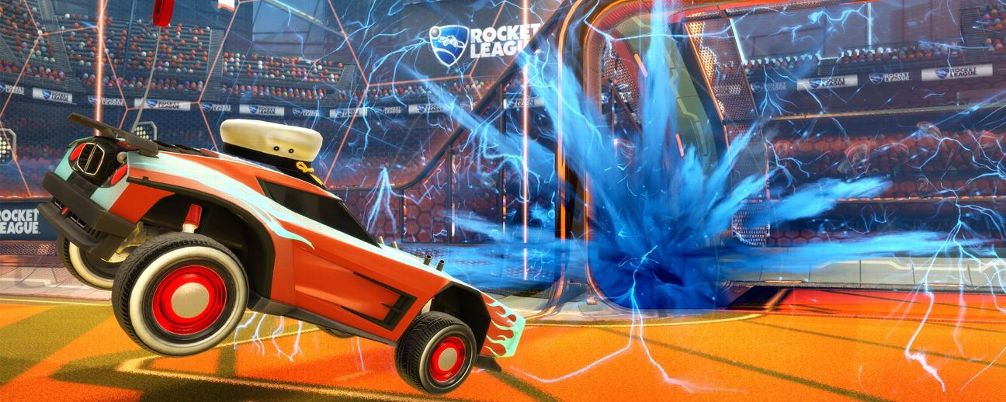
\includegraphics[scale=0.3]{imagens/rocketleague.jpg}
	\caption{\small \textit{Efeitos de fumaça em Rocket League} (Fonte: ESPN, 2016)}
	\label{fig:rocketleague}
\end{figure}

Agora, os vértices passam por uma série de processamentos fixos, o primeiro deles sendo o \textit{transform feedback}. As primitivas geradas anteriormente podem ser armazenadas e recuperadas em \textit{buffer objects}, memórias alocadas pelo programa OpenGL. Isso possibilita que a informação em uso não precise transitar entre a memória RAM e a GPU, diminuindo o tempo de processamento. É útil em sistemas de partículas, por exemplo, onde é necessário simular um grande número de objetos que agem de uma maneira pré-determinada, como a fumaça de uma explosão (figura \ref{fig:rocketleague}).

\begin{figure}[H]
	\begin{subfigure}[b]{0.4\textwidth}
		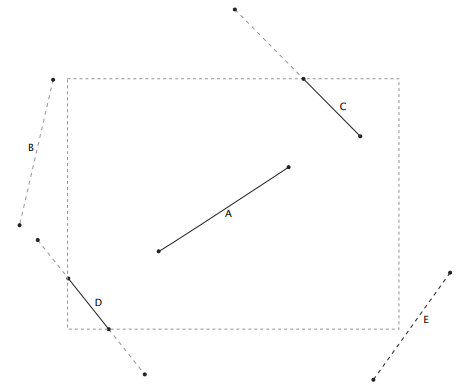
\includegraphics[width=\textwidth]{imagens/line-clipping.png}
		\caption{\textit{Clipping de linha}}
		\label{fig:lineclipping}
	\end{subfigure}
	\hfill
	\begin{subfigure}[b]{0.4\textwidth}
		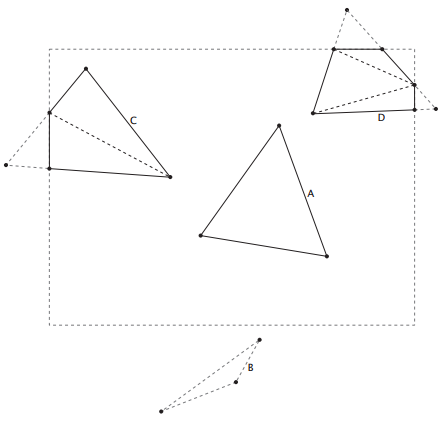
\includegraphics[width=\textwidth]{imagens/triangle-clipping.png}
		\caption{\textit{Clipping de triângulo} }
		\label{fig:triangleclipping}
	\end{subfigure}
	\caption{\textit{Clipping} (Fonte: WRIGHT, HAEMEL, 2016)}
\end{figure}
	
O próximo passo é o \textit{clipping}, onde são determinadas quais primitivas irão aparecer ou não na tela do programa. É possível definir dois tipos de projeção: ortográfica e em perspectiva. Ambas criam formas no espaço em formato de tronco de paralelepípedo e pirâmide, respectivamente. Pontos isolados fora das coordenadas especificadas são descartados automaticamente. Nas figuras \ref{fig:lineclipping} e \ref{fig:triangleclipping}, podemos notar que as linhas e os triângulos C e D seriam parcialmente inclusos na visualização. Nesse caso são geradas novas primitivas que comportam somente as partes que aparecerão no resultado final (OPENGL, 2016d). 

\begin{figure}[H]
	\begin{subfigure}[b]{0.4\textwidth}
		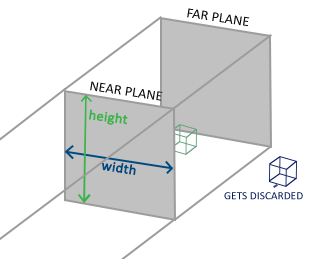
\includegraphics[width=\textwidth]{imagens/orthographic_frustum.png}
		\caption{\textit{Projeção ortográfica} (Fonte: Learn OpenGL, 2016)}
		\label{fig:ortofrustum}
	\end{subfigure}
	\hfill
	\begin{subfigure}[b]{0.4\textwidth}
		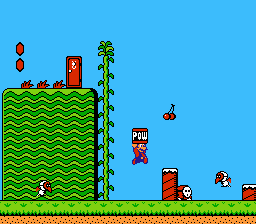
\includegraphics[width=\textwidth]{imagens/mariobros2.png}
		\caption{\textit{Jogo Super Mario Bros 2, projeção ortográfica} (Fonte: Wikipédia, 2016)}
		\label{fig:mariobros2}
	\end{subfigure}
	\caption{Projeção ortográfica}
\end{figure}

Na projeção ortográfica (figura \ref{fig:ortofrustum}) definimos largura, altura e comprimento da projeção. É útil na visualização de elementos 2D, como desenhos técnicos e jogos de plataforma, uma vez que as coordenadas são mapeadas diretamente na tela, não havendo distorção.

\begin{figure}[H]
	\begin{subfigure}[b]{0.4\textwidth}
		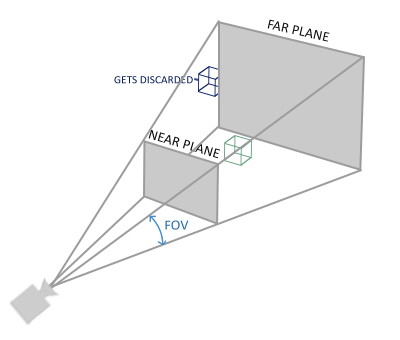
\includegraphics[width=\textwidth]{imagens/perspective_frustum.png}
		\caption{\textit{Projeção em perspectiva} (Fonte: Learn OpenGL, 2016)}
		\label{fig:perspfrustum}
	\end{subfigure}
	\hfill
	\begin{subfigure}[b]{0.4\textwidth}
		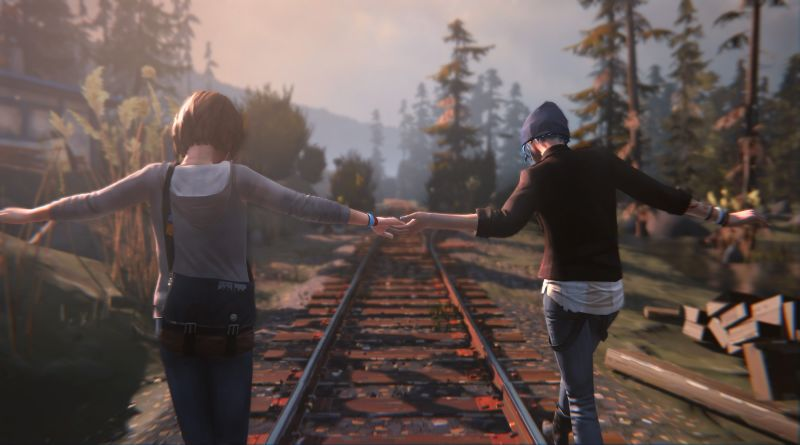
\includegraphics[width=\textwidth]{imagens/life-is-strange.jpg}
		\caption{\textit{Jogo Life is Strange, projeção em perspectiva} (Fonte: Kotaku, 2016)}
		\label{fig:lifeisstrange}
	\end{subfigure}
	\caption{Projeção em perspectiva}
\end{figure}

Na projeção em perspectiva é criada a ilusão de distância, onde objetos mais distantes são renderizados menores que objetos mais próximos. Na figura \ref{fig:lifeisstrange}, podemos observar que os trilhos do trem convergem para o centro da imagem a medida que se distancia do observador. Esse efeito é causado através da equação \ref{eq:perspectiveprojection}, onde $x$, $y$ e $z$ representam as coordenadas de cada vértice e $w$ é um componente


\begin{equation}
	x = 
	\begin{pmatrix} 
		\frac{x}{w} \\
		\frac{y}{w} \\
		\frac{z}{w} 
	\end{pmatrix}
	\label{eq:perspectiveprojection}
\end{equation}
